
\section{Generative Model of Container Contents}
\begin{frame}
  \frametitle{The Problem}
  \begin{center}
    \vspace{-0.13in}
    Set of containers: $\{c_l\}$

    \spL[3-unknown-containers]

    Set of object types: $\{t_i\}$

    \spL[shape-universe-small]

    We want to find an object of type $q$ (the query type).

    \spL[blue-circle]

  \end{center}
\end{frame}

\begin{frame}
  \frametitle{Where is \spM[blue-circle]?}
  \begin{center}
    \spL[3-partially-observed-containers]

    \vspace{0.3in}

    Given that we have observed objects of types $\{t_{o_j}\}$ \\
    in container $c$, what is $\mathrm{P}(q \in c \, | \, \{t_{o_j}\})$ ?
  \end{center}
\end{frame}

\begin{frame}
  \frametitle{Composition of a container ($\theta$)}
  \begin{columns}
    \begin{column}{0.7\textwidth}
      \begin{center}
        \spM[shape-universe-small]\\
        \hspace{0.1in} 1 \hspace{0.2in} 2 \hspace{0.08in} 3 \hspace{0.08in} 4

        \begin{equation*}
          \theta' = (1, 2, 1, 3)
        \end{equation*}

        \begin{equation*}
          \theta = \frac{\theta'}{\norm{1}{\theta'}}
        \end{equation*}

        \begin{equation*}
          \theta = \Big ( \frac17, \frac27, \frac17, \frac37 \Big )
        \end{equation*}
      \end{center}
    \end{column}
    \begin{column}{0.3\textwidth}
      \spL[1-observed-container]
    \end{column}
  \end{columns}
\end{frame}

\begin{frame}
  \frametitle{Prior on Composition ($\theta$)}
  \begin{center}
    We need some prior probability distribution on $\theta$.
    \vspace{0.3in}

    A Dirichlet distribution is a common choice for this kind of application.
    However, the Dirichlet distribution doesn't have enough degrees of freedom to represent co-occurrences.
  \end{center}
\end{frame}

\begin{frame}
  \frametitle{Logistic Normal Prior on Composition ($\theta$)}
  \begin{center}
    \begin{equation*}
      \theta = ( \theta_1, \theta_2, \dots \theta_T )
    \end{equation*}

    \begin{equation*}
      \eta \sim \mathcal{N}(\mu, \Sigma)
    \end{equation*}

    $\sigma(\eta)$ transforms the normally distributed $\eta \in \mathbb{R}^T$ \\
    to $\theta \in \mathbb{R}_+^T$ such that $\norm{1}{\theta} = 1$.

    \begin{equation*}
      \theta_i = \sigma(\eta_i) = \frac{e^{\eta_i}}{\sum_{k=1}^{T}e^{\eta_k}}
    \end{equation*}
  \end{center}
\end{frame}

\begin{frame}
  \frametitle{Logistic Normal Prior on Composition ($\theta$)}
  \begin{center}
    \vspace{-0.4in}
    \begin{equation*}
      \eta \sim \mathcal{N}(\mu, \Sigma)
    \end{equation*}
    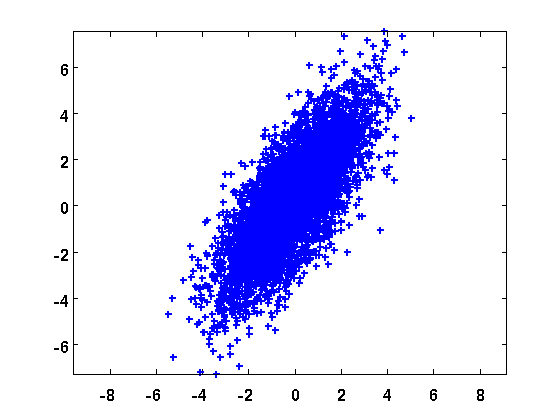
\includegraphics[scale=0.6]{img/log-normal-figs/normal-1.png}
  \end{center}
\end{frame}

\begin{frame}
  \frametitle{Logistic Normal Prior on Composition ($\theta$)}
  \begin{center}
    \vspace{-0.3in}
    \begin{equation*}
      \theta_i = \sigma(\eta_i) = \frac{e^{\eta_i}}{\sum_{k=1}^{T}e^{\eta_k}}
    \end{equation*}

    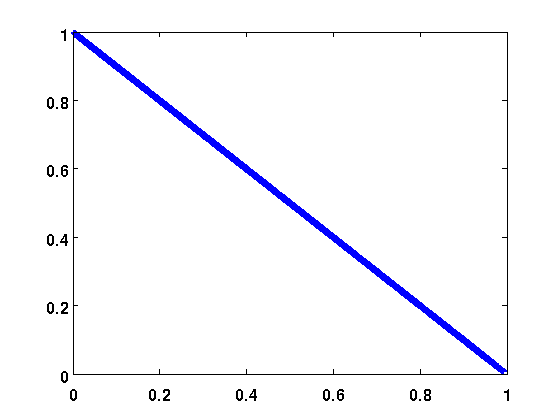
\includegraphics[scale=0.5]{img/log-normal-figs/log-normal-1.png}
  \end{center}
\end{frame}

\begin{frame}
  \frametitle{Logistic Normal Prior on Composition ($\theta$)}
  \begin{center}
    Histogram of $\theta_i$
    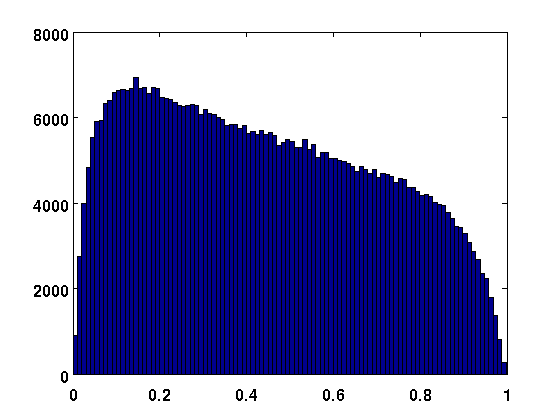
\includegraphics[scale=0.6]{img/log-normal-figs/hist-1.png}
  \end{center}
\end{frame}

\begin{frame}
  \frametitle{Logistic Normal Prior on Composition ($\theta$)}
  \begin{center}
    \vspace{-0.4in}
    \begin{equation*}
      \eta \sim \mathcal{N}(\mu, \Sigma)
    \end{equation*}
    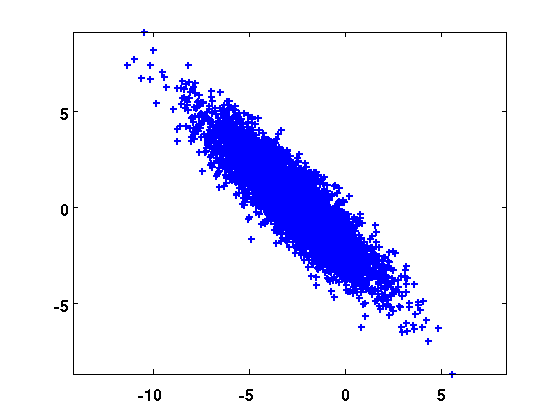
\includegraphics[scale=0.6]{img/log-normal-figs/normal-2.png}
  \end{center}
\end{frame}

\begin{frame}
  \frametitle{Logistic Normal Prior on Composition ($\theta$)}
  \begin{center}
    \vspace{-0.3in}
    \begin{equation*}
      \theta_i = \sigma(\eta_i) = \frac{e^{\eta_i}}{\sum_{k=1}^{T}e^{\eta_k}}
    \end{equation*}

    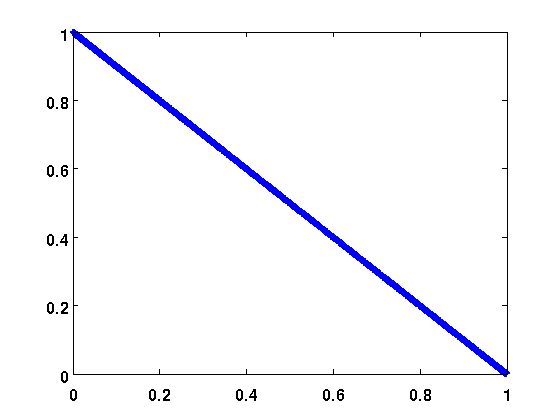
\includegraphics[scale=0.5]{img/log-normal-figs/log-normal-2.png}
  \end{center}
\end{frame}

\begin{frame}
  \frametitle{Logistic Normal Prior on Composition ($\theta$)}
  \begin{center}
    Histogram of $\theta_i$
    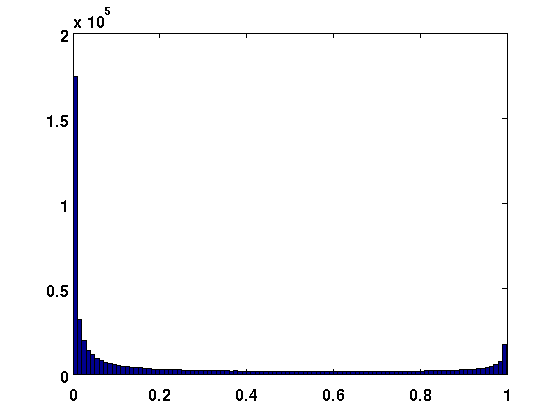
\includegraphics[scale=0.6]{img/log-normal-figs/hist-2.png}
  \end{center}
\end{frame}

\begin{frame}
  \frametitle{Inverse of Logistic Transformation}
  \begin{center}
    \begin{equation*}
      \eta \sim \mathcal{N}(\mu, \Sigma)
    \end{equation*}

    \begin{equation*}
      \theta_i = \sigma(\eta_i) = \frac{e^{\eta_i}}{\sum_{k=1}^{T}e^{\eta_k}}
    \end{equation*}

    \begin{equation*}
      \eta_i = \sigma^{-1}(\theta_i)
    \end{equation*}

    \begin{equation*}
      \eta_i \propto \ln \theta_i
    \end{equation*}

    WTF! THIS DOESN'T SEEM TO WORK! \\
    HELP ME PROFESSOR WILLIAMS! YOU'RE MY ONLY HOPE!
  \end{center}
\end{frame}

\begin{frame}
\frametitle{Spacial constraints on container contents}
\begin{center}
The size of the unseen component of a container restricts what objects could be
inside it.
\vspace{3em}

Incorporate these spacial constraints to calculate 
$\mathbb{P}(q \in c_l|\{t_{o_j}\})$
from samples of $\theta$
\end{center}
\end{frame}

